%%%%%%%%%%%%%%%%%%%%%%%%%%%%%%%%%%%%%%%%%
% Thin Sectioned Essay
% LaTeX Template
% Version 1.0 (3/8/13)
%
% This template has been downloaded from:
% http://www.LaTeXTemplates.com
%
% Original Author:
% Nicolas Diaz (nsdiaz@uc.cl) with extensive modifications by:
% Vel (vel@latextemplates.com)
%
% License:
% CC BY-NC-SA 3.0 (http://creativecommons.org/licenses/by-nc-sa/3.0/)
%
%%%%%%%%%%%%%%%%%%%%%%%%%%%%%%%%%%%%%%%%%

%----------------------------------------------------------------------------------------
%	PACKAGES AND OTHER DOCUMENT CONFIGURATIONS
%----------------------------------------------------------------------------------------

\documentclass[a4paper, 11pt]{article} % Font size (can be 10pt, 11pt or 12pt) and paper size (remove a4paper for US letter paper)
\usepackage{listings}   
\usepackage{amsmath}
\usepackage{wrapfig} % Allows in-line images
\usepackage{graphicx}
\usepackage{mathpazo} % Use the Palatino font
\usepackage[T1]{fontenc} % Required for accented characters
\usepackage{floatrow}
\usepackage{lmodern}
\usepackage{graphicx}
\usepackage{amsthm}
\usepackage{float}
\newtheorem*{theorem*}{Theorem}
\newtheorem*{corollary*}{Corollary}
\usepackage{lingmacros}
\linespread{1.05} % Change line spacing here, Palatino benefits from a slight increase by default

\makeatletter
\renewcommand\@biblabel[1]{\textbf{#1.}} % Change the square brackets for each bibliography item from '[1]' to '1.'
\renewcommand{\@listI}{\itemsep=0pt} % Reduce the space between items in the itemize and enumerate environments and the bibliography

\renewcommand{\maketitle}{ % Customize the title - do not edit title and author name here, see the TITLE block below
\begin{flushright} % Right align
{\LARGE\@title} % Increase the font size of the title

\vspace{50pt} % Some vertical space between the title and author name

{\large\@author} % Author name
\\\@date % Date

\vspace{40pt} % Some vertical space between the author block and abstract
\end{flushright}
}

%----------------------------------------------------------------------------------------
%	TITLE
%----------------------------------------------------------------------------------------

\title{\textbf{How to Quantitate a Markov Chain?}\\ % Title
Stochostic project 1} % Subtitle

\author{\textsc{Chi-Ning,Chou  Wei-chang,Lee} % Author
\\{\textit{PROFESSOR RAOUL NORMAND }}} % Institution

\date{\today} % Date

%----------------------------------------------------------------------------------------

\begin{document}

\maketitle % Print the title section

%----------------------------------------------------------------------------------------
%	ABSTRACT AND KEYWORDS
%----------------------------------------------------------------------------------------

%\renewcommand{\abstractname}{Summary} % Uncomment to change the name of the abstract to something else

\begin{abstract}
In this project, we want to quantitatively evaluate a Markov chain. In the beginning, we give a simple introduction to Information Theory ,and then focus on the inequality of mutual information of a Markov process. In the main part of this project, we try to prove the second law of thermodynamics in Markov chains, and derived some quantities to measure the distance between current state and the stationary state. We will use Matlab to simulate Bernoulli-Laplace model to bridge realistic world with our quantitative approach.Finally, we will comment on the second law of thermodynamics under other entropy definition.
\end{abstract}

\hspace*{5,6mm}\textit{Keywords:} Entropy , Markov chain , Kullback-Leibler divergence , Bernoulli-Laplace model , Thermodynamics % Keywords

\vspace{30pt} % Some vertical space between the abstract and first section

%----------------------------------------------------------------------------------------
%	ESSAY BODY
%----------------------------------------------------------------------------------------

\section*{Introduction}

\paragraph{}
In classical thermodynamics, people like to use entropy to evaluate the structural tendency in a system,which is the log number of microstates.
While the well known Second Law of Thermodynamics claims that in a natural thermodynamic process, the
entropy in the participated system will increase, we want to find out whether there also exists some properties
in a Markov chain that quantitatively reveal the structural tendency in the system.

\paragraph{}
In the beginning, we applied the definition of entropy that Claude Shannon used in Information theory to
construct the entropy in a Markov chain. However, after deducing some corresponding results, we found that
such definition does not elegantly reveal the tendency in the system. As a result, we surveyed and tried
other models to describe the structure of a Markov chain, rethinking how to interpret Shannon's entropy
in a Markov chain.

\paragraph{}
In this report, we will first apply Shannon's entropy to examine the corresponding results in a Markov
chain. Next, some other structural properties will be introduced. In the third part of the report, we will use
a simple urn problem which is known as Bernoulli-Laplace model to demonstrate the properties we prove in this project. And we will give some
comments on each structural properties and discuss the difference of Shannon's entropy and the entropy in
thermodynamic at last.%------------------------------------------------

\section*{Information Theory Preliminaries}
\paragraph{}
In this section, we briefly introduce Shannon entropy, mutual information, Kullback-liebler divergence  and some useful results such as Kullback-liebler divergence of a Markov chain will always decrease as time goes by.
\paragraph{Shannon Entropy}
The entropy of a random variable is a measure of the uncertainty of itself. It is a measure of the amount of information required on the average to describe this random variable.\\
The entropy H(x) of a discrete random variable X is defined by:
\begin{align*} 
 H(X)	&= -\sum_{x\in X}p(x)\log p(x)\\
&=E_p[\frac{1}{\log p(x)}]
\end{align*}

\paragraph{}
And the conditional entropy is given by
\begin{align*} 
 H(Y|X)	&= \sum_{x\in X}p(x)H(Y|X=x)\\
 &=-\sum_{x\in X}p(x)\sum_{y\in Y}p(y|x)\log p(y|x)\\
 &=-\sum_{x\in X}\sum_{y\in Y}p(x,y)\log p(y|x)
 \end{align*}

\paragraph{}
For a pair of discrete random variable X and Y:
\begin{align*} 
 H(X,Y)	&= -\sum_{x\in X}\sum_{y\in Y}p(x,y)\log p(x,y)\\
        &= -\sum_{x\in X}\sum_{y\in Y}p(x,y)\log p(x)p(y|x)\\
        &=H(X)+H(Y|X)
\end{align*}
When it comes to continuous random variable, just substitutes integral for summation. 
\begin{theorem*}
\emph{(Uniform Distribution Maximize Shannon Entropy)}\\
Given a finite state Markov chain, it's Shannon entropy is maximized if and only if current distribution is uniform.
\end{theorem*}
\paragraph{}
The theorem gives us an intuition that the entropy of a Markov chain is maximized when the probability of every microscopic state to show up  is the same! That is, if we start the stochastic process with uniform distribution, the entropy is maximized in the very beginning. So, it's clearly that the {\it Second Law of Thermodynamics} does not hold under Shannon entropy!

\paragraph{Kullback-liebler divergence}
We can use the definition above to derive relative entropy, which is a measure of distance between two distributions. The relative entropy or Kullback-liebler divergence between two pmf p(x) and q(x) is defined as:
\begin{align*} 
 D(p||q) &= -\sum_{x\in X}p(x)\log \frac{p(x)}{q(x)}\\
         &=E_p[\log \frac{1}{q(x)}]-E_p[\log \frac{1}{p(x)}]
 \end{align*}
\paragraph{}
The Kullback-Leibler divergence measures the expected number of extra bits required to code samples from P when using Q.
 It is non-negative and asymmetric : 
\begin{align*} 
 D(p||q)\neq D(q||p)\geq 0
  \end{align*}
  
\begin{theorem*}
\emph{(Kullback-liebler Divergence)}\\
For a Markov chain with unique stationary distribution, the Kullback-liebler divergence between the distribution of each step and the stationary distribution will monotonically decrease to zero.
\end{theorem*} 
\paragraph{}
To prove this theorem, we first need the following lemma.
\paragraph{Lemma}
If $u_n$ and $u'_n$ are two distribution on the same Markov chain at step n. Then, $D(u_n||u'_n)$ is monotonically decreasing.
\begin{proof}
Denote the corresponding distribution of $\{u_n\}$ and $\{u'_n\}$ by $p$ and $q$. This can be easily shown by observing,
\begin{align*}
D&(p(x_n,x_{n+1})||q(x_n,x_{n+1}))\\
&=D(p(x_n)||q(x_n)) + D(p(x_n|x_{n+1})||q(x_n|x_{n+1})) &chain ~rule \\
&=D(p(x_{n+1})||q(x_{n+1})) + D(p(x_{n+1}|x_n)||q(x_{n+1}|x_n))
\end{align*}
Since $p(x_{n+1}|x_n)=q(x_{n+1}|x_n)$, it's straight forward that
\begin{equation*}
D(p(x_{n+1}|x_n)||q(x_{n+1}|x_n)) = 0
\end{equation*}
Thus,
\begin{equation*}
D(p(x_n||q(x_n)) \geq D(p(x_{n+1})||q(x_{n+1}))
\end{equation*}
\end{proof}
Finally, to prove the monotonically decreasing of Kullback-liebler divergence between current distribution and stationary distribution, just simply set $q=\pi$ then the result is shown.
Any step distribution gets closer and closer to the unique stationary distribution as time goes by. $D(u_{n}||\pi)$ is a monotonically non-increasing non-negative sequence and thus have a limit $D(\pi||\pi)=0$.  
\paragraph{Mutual Information}
The mutual information I(X;Y) is the relative entropy between the joint distribution and the product distribution p(x).p(y):
\begin{align*} 
I(X;Y)=&= -\sum_{x,y}p(x,y)\log \frac{p(x,y)}{p(x)p(y)}\\
       &=-\sum_{x,y}p(x,y)\log \frac{p(x|y)}{p(x)}\\
       &=H(X)-H(X|Y)\geq 0\\
 \end{align*}
\paragraph{}
The mutual information I(X;Y) is the reduction in the uncertainty of X due to the knowledge of Y. It is easily to derive following property.
\begin{align*} 
I(X;Y)=I(Y;X)\\
I(X;X)  =H(X;X)\\
H(X)\geq H(X|Y)
 \end{align*}

 
\paragraph{}
We can use a Venn diagram to visualize the relationship between the entropy concept we discussed above:
\begin{figure}[ht]
\begin{center}
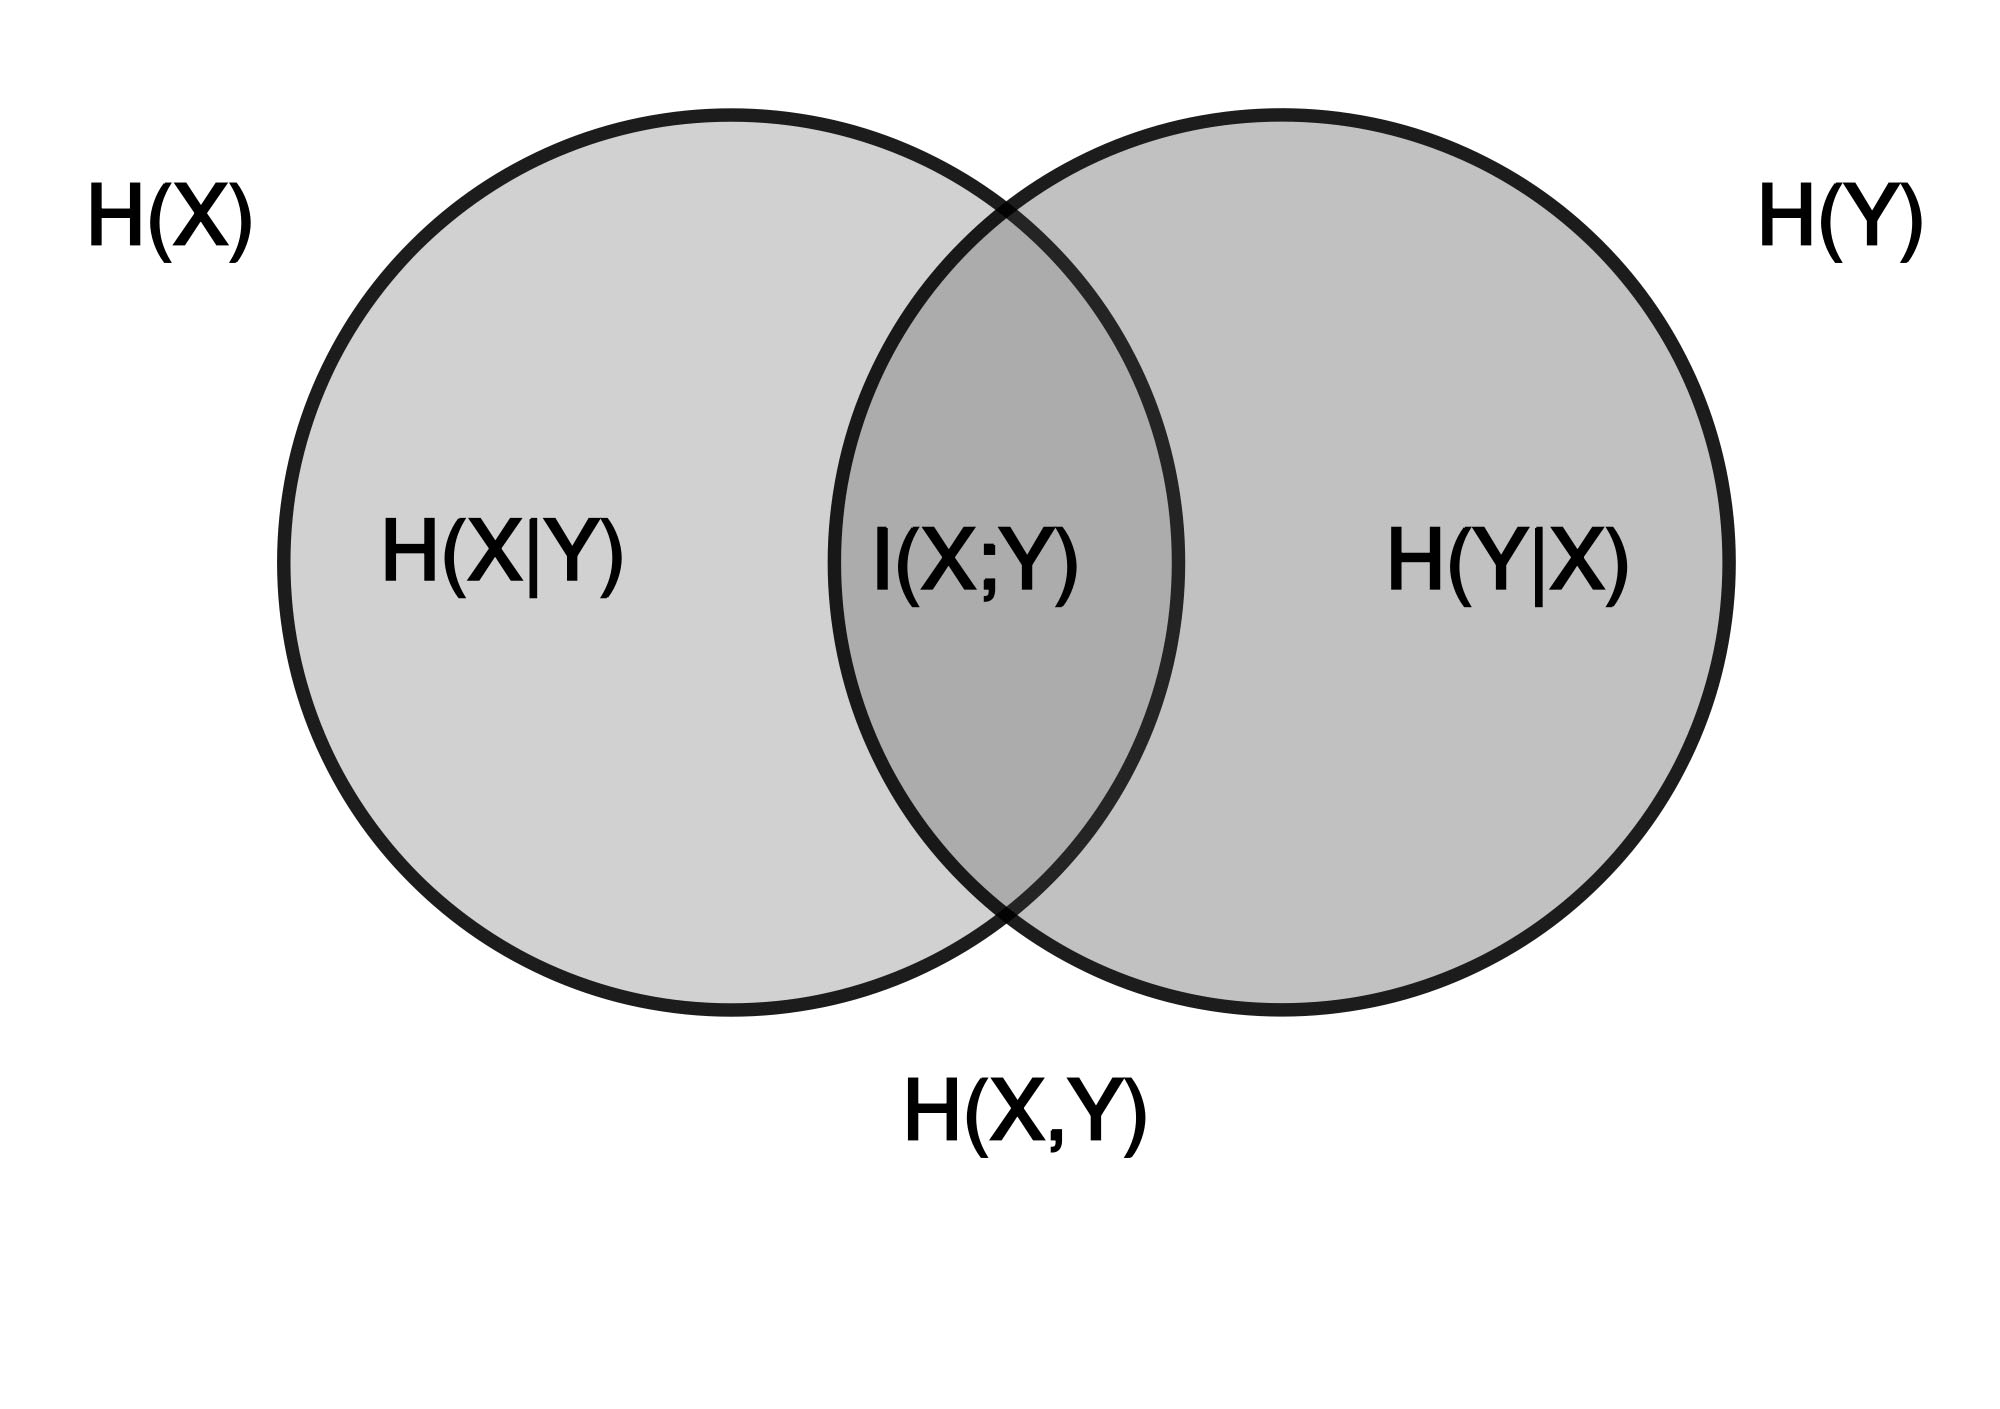
\includegraphics[width=2 in]{venn.jpg}
\vskip 5 pt
\caption{Venn's diagram for mutual information}
\end{center}
\end{figure}
%------------------------------------------------
\subsection*{Data processing Inequlity}

\paragraph{}
Under simple Markov assumption, We can show that no clever manipulation of the data can improve the inferences that can be made from the original data.\\
$If ~X\rightarrow Y\rightarrow Z ~forms ~a ~Markov ~chain, ~then ~I(X;Y)\geq I(X;Z)$
\begin{align} 
I(X;Y,Z)&=I(X;Z)+I(X;Y|Z)\\
       &=I(X;Y)+I(X;Z|Y)     
 \end{align}
\paragraph{}
First focus on $I(X;Z|Y)$, we notice that:
\begin{align*} 
I(X;Z|Y)&=H(X\vert Y)-H(X|Z,Y)\\
       &=E_P(x,y,z)\log \frac{p(x,z|y)}{p(x|y).p(z|y)}\\
       &=E_P(x,y,z)\log \frac{\frac{p(x,y,z)}{p(y)}}{p(x|y).p(z|y)}\\
       &=E_P(x,y,z)\log \frac{\frac{p(x,y)p(z|y)}{p(y)}}{p(x|y).p(z|y)}\\
       &=E_p(x,y,x)\log 1  
       &=0
 \end{align*}
\paragraph{}
From (1) and (2) we can easily get $I(X;Y)\geq I(X;Z)$, Z can be written as a function of Y, thus we cannot increase the mutual information of X and Y by transforming Y to Z. Note that $I(X;Y|Z)\leq I(X;Y)$ can be derived from (1) and (2), which means that the dependency of X and Y is decreased by observing Z. It is because that transition matrix is invertible, $Z\rightarrow Y\rightarrow X$ also forms a Markov chain. Z reveals some information about X and Y.
\paragraph{}
The conclusion of no clever manipulation of the data can improve the inferences may lead to misconception that the shuffle do not increase randomness of the cards. We can prove that it is not true if shuffle method T and card positions X are independent :
\begin{align*} 
H(TX)&\geq H(TX|T)&condition~reduce~entropy\\
       &=H(T^{-1}TX|T)&we~know~T^{-1}~conditioning~T\\
       &=H(X|T)&independence \\
       &=H(X)  
 \end{align*}
\paragraph{}
By a further application of data processing inequality to a stationary Markov chain $X_1\rightarrow X_{n-1}\rightarrow X_n$, we have: 
\begin{align*} 
I(X_1;X_{n-1})&\geq I(X_1;X_n)\\
H(X_{n-1})-H(X_{n-1}|X_1)&\geq H(X_{n})-H(X_{n}|X_1)&&expand\\ 
H(X_{n-1})&=H(X_{n})&&stationary
\end{align*}

\paragraph{}

\begin{theorem*}
\emph{(Conditional Entropy given Initial Distribution)}\\
If $\{X_n\}$ is a stationary Markov chain, then
\begin{equation*}
H(X_{n+1}\vert X_1) \geq H(X_n\vert X_1) \quad \forall n
\end{equation*}
Moreover, the conditional entropy given initial distribution will converge to the Shannon entropy of the stationary distribution.
\end{theorem*}

\paragraph{}
The conditional entropy $H(X_{n}|X_{1})$ increases with n. Thus the conditional uncertainty of the future increases. Note that since conditioning reduces entropy, $H(X_{n}|X_{1})$ will be bounded by $H(X_{n})$ and since $H(X_{n}|X_{1})$  is non-decreasing with n. It will finally reach a limit, which is the entropy of stational distribution $H(X_{\pi})$   
\section*{Entropy and the Second Law of Thermodynamics}
\paragraph{}
Since we can model the evolution of an isolated system as a Markov chain with transition matrix obeying the physical laws governing the system, we can use Shannon entropy to quantify the degree of chaos of this system. After studying the basic properties of Shannon entropy, we further work on figuring out whether the statement of the Second Law of Thermodynamics still holds true, that is the entropy of an isolated system is always nondecreasing, and whether the physical meaning makes sense.\\

In the following, we are going to deduce some related theorems to the Second Law of Thermodynamics.

\begin{theorem*}
\emph{(Time related Entropy of Markov Chain)}\\
The Shannon entropy of most Markov chain does not necessarily decrease with time.
\end{theorem*}

According to the previous lemma, we know that Shannon entropy is maximized when it is uniform distribution. Thus, if the stationary distribution of a Markov chain is not uniform, if the initial distribution is uniform, the Shannon entropy will decrease in the beginning, which violate the Second Law of Thermodynamics.

\begin{theorem*}
\emph{(Monotonically Decreasing of KL-Divergence)} \\
Suppose a Markov chain has an unique stationary distribution and is irreducible, then the KL-distance between current distribution and the stationary distribution will monotonically decreasing. That is,
\begin{equation*}
D(\mu_{n+1}||\pi)\leq D(\mu_n||\pi) \\
\end{equation*}
\end{theorem*}

\begin{corollary*}
\emph{(Non-decreasing entropy condition)} \\
Suppose a Markov chain has an uniform stationary distribution ,or  a doubly stochastic transition matrix. The entropy is non-decreasing over time.
\begin{equation*}
D(\mu_{n}||\pi)=log|\mathcal{X}|-H(\mu_{n})= log|\mathcal{X}|-H(X_{n})\\
\end{equation*}
\end{corollary*}

\paragraph{}
The  monotonic  decrease  in  KL-Divergence implies  a 
monotonic  increase  in  entropy when the stationary distribution is uniform. The  fact resonates closely with 
Boltzmann entropy in statistical thermodynamics, since it is defined as the log number of microscopic states.       

\begin{theorem*}
\emph{(Conditional Entropy)}\\
The conditional entropy of a Markov chain will monotonically decrease.
\end{theorem*}
\paragraph{}
The theorem follows the properties that Shannon entropy in the previous section. However, the fact that relative entropy always decreases have no straight forward relation to Shannon entropy.

\paragraph{}
To sum up, the Second Law of Thermodynamics basically doesn't hold true when applying Shannon entropy into our observed system. However, there are still exist good quantity method which has monotonically property. The first one is KL-distance between current distribution and the stationary distribution, which will monotonically decrease. And the second one is conditional entropy of current distribution given the initial distribution, which will monotonically increase.

\section*{Simulation on Bernoulli-Laplace model}

\paragraph{}
In this section, we use Erenfest model to demonstrate the concepts and the results in the previous part.

\paragraph{Model Setting}
First, let's construct the model settings.
\begin{itemize}
\item There are two urns: A, B in our system.
\item Each urn contains $n$ balls in the beginning. And the ball in urn A is black while the ball in urn B is white.
\item In each step, we take one ball with uniform probability from each urn and make an exchange.
\end{itemize}
\begin{figure}[!h]
\begin{floatrow}
\ffigbox{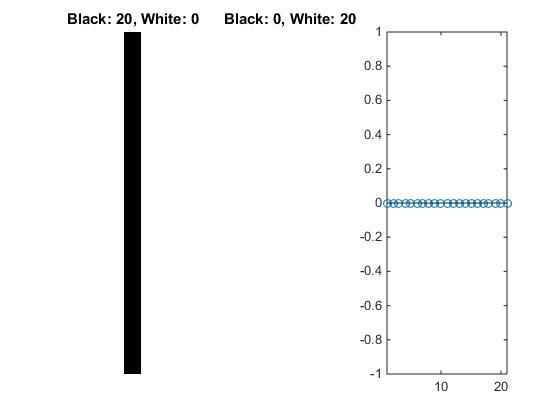
\includegraphics[scale = 0.3]{problemsetting_1.jpg}}{\caption{Initial setting}\label{case1}}
\ffigbox{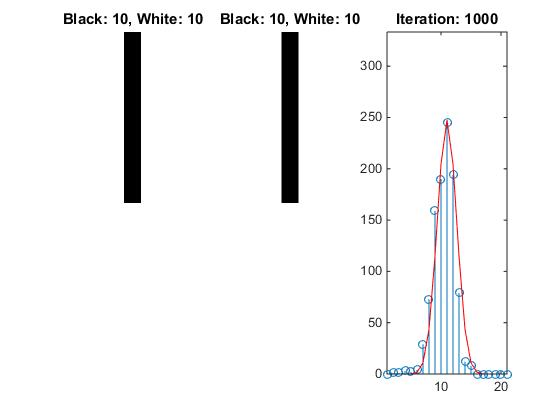
\includegraphics[scale = 0.3]{problemsetting_2.jpg}}{\caption{After 1000 iterations}\label{zoom}}
\end{floatrow}
\end{figure}


\paragraph{Properties}
With these initial settings, we can simply find out that this system is a Markov chain and easily derive the below properties of this process:
\begin{itemize}
\item The state space $S = \{S_i\vert i=0,1,...,n\}$, where $S_i$ refers to the configuration that urn A contains $i$ black balls and $n-i$ white balls, while urn B contains $n-i$ black balls and $i$ white balls.
\item The transition probability is
\begin{equation}
P(X_n = i,X_{n+1} = j) = \left\{
\begin{array}{lcl}
{(\frac{i}{n})^2} & if \quad j = i-1\quad and\quad i \geq 1 \\
{\frac{2i(n-i)}{n^2}} & if \quad j = i\quad and\quad 1 \leq i \leq n-1 \\
{(\frac{n-i}{n})^2} & if \quad j = i+1 \quad and \quad i\leq n-1 \\
{1} & if \quad i=0, j=1 \quad or \quad i=n,j=n-1
\end{array} 
\right.
\end{equation}

\item The stationary distribution is hypergeometric distribution
\begin{equation}
\pi(i)=\frac{{20 \choose i}{20 \choose 20-i}}{{40 \choose20}}
\end{equation} 
\end{itemize}

\paragraph{}
In the following simulation, we set the number of balls in each urn to $20$ and observe the: Shannon entropy, Kullback-liebler divergence  to the stationary distribution and conditional entropy given initial distribution.
\hspace*{2mm} Also, we consider two different initial distribution: uniform  distribution and random  distribution.

\paragraph{}
We can see the following results:
\begin{enumerate}
\item In the first graph, it's clearly that the distribution after 40 iterations is very close to the stationary distribution.
\item In the second graph, the Kullback-liebler divergence  between current distribution and the stationary distribution is monotonically decreasing.
\item In the third graph, we can see that the Shannon entropy(red curve) is decreasing while the conditional entropy given initial distribution is monotonically increasing.
\end{enumerate}

\paragraph{}
First, consider the uniform initial distribution. Note that, the Shannon entropy is maximized when the the distribution is uniform.\\
\hspace*{2mm} The simulation results are in the following figure:
\begin{figure}[H]
\begin{center}
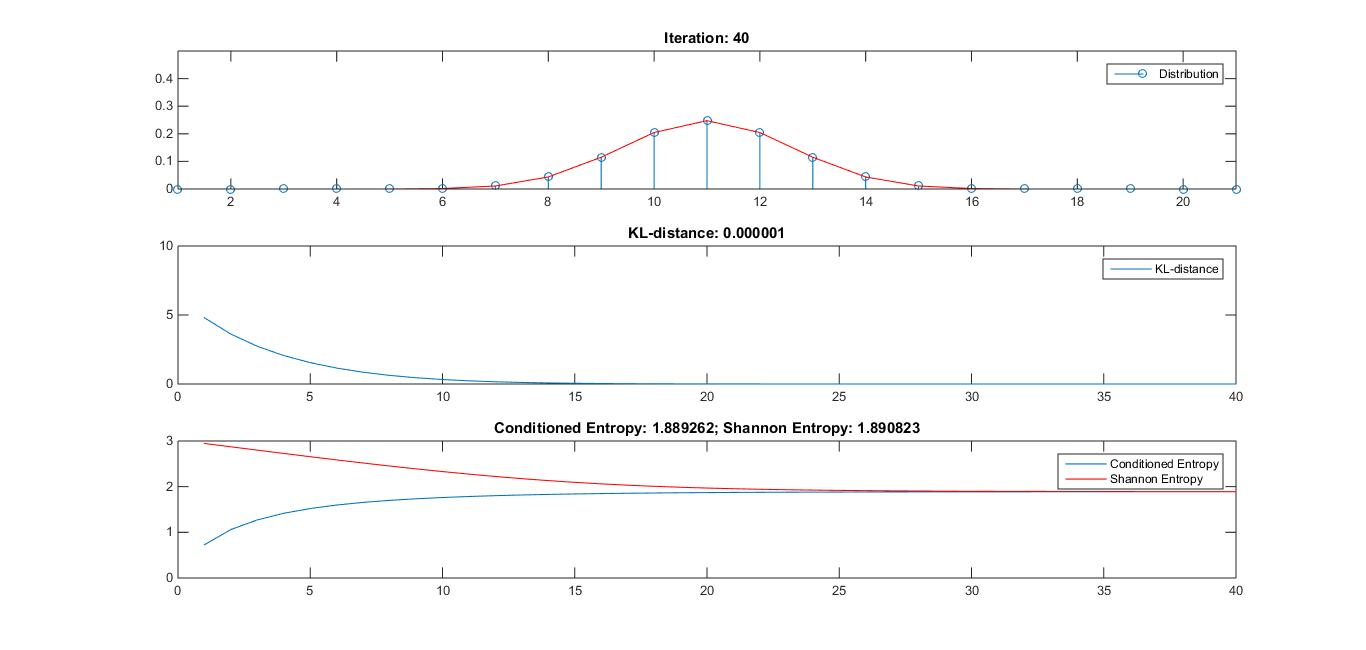
\includegraphics[scale=0.27]{uniform.jpg}
\end{center}
\caption{Start with uniform distribution}
\end{figure}

\paragraph{}
Then we randomly choose the initial distribution and get the following results:
\begin{figure}[H]
\begin{center}
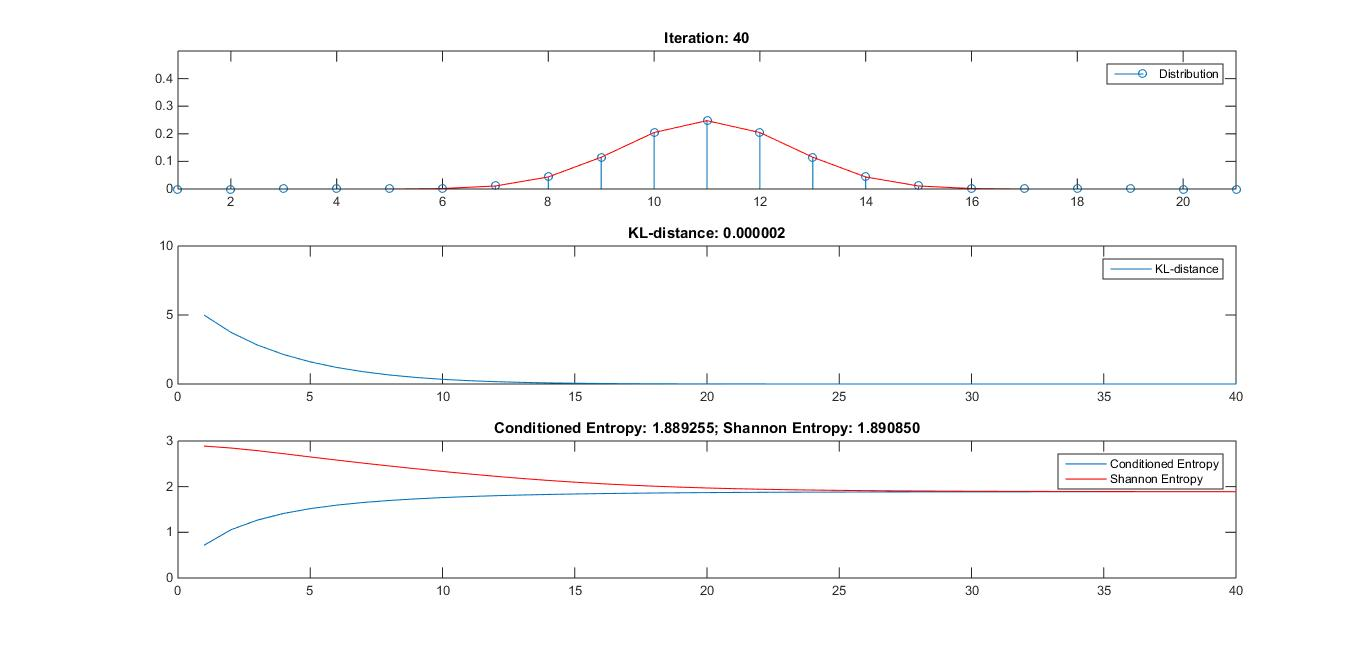
\includegraphics[scale=0.27]{random.jpg}
\end{center}
\caption{Start with random initial distribution}
\end{figure}

\section*{Conclusion}
\paragraph{}
Based on the ideas in information theory, we tried to apply various quantities to evaluate a Markov chain in light of demonstrating {\it The Second Law of Thermodynamics}. First, we find that although Shannon entropy sometimes perfectly describe a stochastic process, it has totally different physical meanings from the classical Boltzmann entropy, which emphasizes on single microscopic state.\\

As a result, we turn to Kullback-liebler divergence  to quantitatively measure an ongoing Markov chain. And it turns out that the Kullback-liebler divergence  between current distribution and stationary distribution will monotonically decreasing to 0 while the chain has an unique stationary distribution.\\

Finally, we showed that the conditional entropy of current distribution given initial distribution   will monotonically increasing to the Shannon entropy of stationary distribution. That is, the future will be more and more difficult to predict from the beginning. However, the uncertainty cannot exceed an upper, which is the entropy of stationary distribution, since conditioning never hurts.\\

After surveying how to apply the concept in Information theory to describe the similar thermodynamic-like behaviour of Markov chain. Now we try to consider the intuition behind this Information theoretical approach.\\

The physical meaning behinds the classical thermodynamic view and information theoretical view have some fundamental difference. For classical thermodynamics, they believe a system will tend to a {\bf single} equilibrium microscopic state. And they admit that they might exist some {\bf fluctuations} near the equilibrium state. This point of view is {\it spatial}, which focus on the deterministic phenomenon.\\

However, for information theorist, the entropy that they are interested in is a description view based on {\bf probabilistic} distribution which they can lately use for modelling a stochastic process. For instance, how to code an article to get the shortest bits to encode it? Which relied further on {\bf distribution of states over time}, but not a deterministic microscopic state information such as the energy of this state.\\
 
In the future, we want to learn more about different modern modelling techniques such as Ising model and Kolmogorov complexity so as to bound the theory with the real environment tighter. After all, using practical mathematical model to map the realistic world to code segments that Turing-recognizable is always a computer scientist wants to do.

%----------------------------------------------------------------------------------------
%	BIBLIOGRAPHY
%----------------------------------------------------------------------------------------



%----------------------------------------------------------------------------------------
\section*{Appendix:  Simulation Code}
\begin{enumerate}
\item main program
\lstset{language=Matlab}        
\begin{lstlisting}[frame=single]  
%% Init
clc;
clear;

n = 20; % number og balls

% transition matrix
A = zeros(n+1,n+1);
A(1,2) = 1;
A(n+1,n) = 1;
for i = 2:n
    A(i,i-1) = (i*i)/(n*n);
    A(i,i+1) = ((n-i)*(n-i))/(n*n);
    A(i,i) = 1 - A(i,i-1) - A(i,i+1);
end
stationary = null(A'-eye(n+1));
stationary = stationary/sum(stationary);

%% Real Simulation
% In this section, we simulate a single trail in the 
% urn problem. That is, we start from an initial 
% state and then using the transition matrix to
% decide the next state of the system.

% Initial state
%   Using the number of balls to record which is the
%   current state
a = n; % urn A
niter = 0; % number of iterations

% image setting
imgA = zeros(n,1);
subplot(1,3,1); imshow(kron(imgA,ones(20)));
imgB = ones(n,1);
title(sprintf('Black: %d, White: %d', a, n-a));
subplot(1,3,2); imshow(kron(imgB,ones(20)));
title(sprintf('Black: %d, White: %d', n-a, a));
% state record
s = zeros(n+1,1);
s(1) = 0;
subplot(1,3,3);
stem(s);
axis([1,n+1,0,niter/3]);

for i = 1:niter
    if rand < a/n % urn A choose black
        if rand <= (n-a)/n % urn B choose black
        else % urn B choose white
            imgA(a) = 1;
            imgB(n-a+1) = 0;
            a = a-1;
        end
    else % urn A choose white
        if rand <= (n-a)/n % urn B choose black
            imgA(a+1) = 0;
            imgB(n-a) = 1;
            a = a+1;
        else % urn B choose white
        end
    end
    
    % update s
    s(n-a+1) = s(n-a+1)+1;
    
    % show result
    if mod(i,5) == 0
        subplot(1,3,1);
        imshow(kron(imgA,ones(20)));
        title(sprintf('Black: %d, White: %d', a, n-a));
        subplot(1,3,2);
        imshow(kron(imgB,ones(20)));
        title(sprintf('Black: %d, White: %d', n-a, a));
        subplot(1,3,3);
        stem(s); hold on;
        axis([1,n+1,0,niter/3]);
        title(sprintf('Iteration: %d', i));
        hold off;
        drawnow;
    end
end

%% Distribution Simulation
% We will focus on three properties:
%   1) Shannon Entropy
%   2) Kullback-liebler divergence 

% Initial state
start_type = 1;
if start_type == 1 % random
    s = rand(1,n+1);
    s = s/sum(s);
elseif start_type == 2 % uniform
    s = ones(1,n+1);
    s = s/sum(s);
end
ss = s; % record initial state distribution

% Transition matrix from first state
B = A;
    
niter = n*2;
e = zeros(niter);
d = zeros(niter);
r = zeros(niter);

figure();
subplot(3,1,1);
stem(s); hold on;
legend('Distribution'); hold off;
axis([1,n+1,0,0.5]);
subplot(3,1,2);
plot(e); hold on;
legend('KL-distance'); hold off;
subplot(3,1,3);
plot(d); hold on;
legend('Conditioned Entropy','Shannon Entropy');
hold off;

for i = 1:niter
    s = s*A;
    d(i) = KL_distance(s',stationary);
    e(i) = entropy(s);
    % relative entropy
    r(i) = relativeentropy(ss,B);
    B = B*A;
    % plot
    subplot(3,1,1); stem(s);
    axis([1,n+1,0,0.5]);
    title(sprintf('Iteration: %d', i));
    legend('Distribution');
    subplot(3,1,2); plot(real(d(1:i))); 
    axis([0,niter,0,10]);
    title(sprintf('KL-distance: %f', d(i)));
    legend('KL-distance');
    subplot(3,1,3); plot(real(r(1:i))); hold on; 
    plot(e(1:i),'r-'); axis([0,niter,0,3]);
    title(sprintf('Conditioned Entropy: %f; ...
    Shannon Entropy: %f', r(i), e(i)));
    legend('Conditioned Entropy', 'Shannon Entropy');
    hold off;
    drawnow; pause(0.1);
end
\end{lstlisting}

\item entropy.m
\begin{lstlisting}[frame=single] 
function [H] = entropy(p)
H = 0;
for i = 1:length(p)
    tmp = -p(i)*log(p(i));
    if ~isnan(tmp) && ~isinf(tmp)
        H = H + tmp;
    end
end
end
\end{lstlisting}

\item KL\_distance.m
\begin{lstlisting}[frame=single] 
function [d] = KL_distance(s, mu)

if length(s) ~= length(mu)
    disp('KL-dis error, different length');
end

d = 0;
for i = 1:length(s)
    tmp = s(i) .* log(s(i)/mu(i));
    if ~isnan(tmp) && ~isinf(tmp)
        d = d+tmp;
    end
end;
end
\end{lstlisting}

\item relativeentropy.m
\begin{lstlisting}[frame=single] 
function [H] = relativeentropy(ss,B)
H = 0;
A = -B.*log(B);
for i = 1:size(A,1)
    for j = 1:size(A,2)
        if isnan(A(i,j))
            A(i,j) = 0;
        end
    end
end
tmp = ss*(A);
for i = 1:length(tmp)
    if ~isnan(tmp(i))
        H = H + tmp(i);
    end
end
end
\end{lstlisting}
\end{enumerate}

\newpage

\bibliographystyle{plain}
\begin{thebibliography}{9}

\bibitem{IT}
\emph{Elements of Information Theory},
Thomas M. Cover, Joy A. Thomas,
John Wiley \& Sons.Inc,
1991.
\bibitem{MARTIN}
\emph{Entropy and the Bernoulli-Laplace Urn Model},
Martin J. Klein,
1956
\end{thebibliography}

\end{document}